\section{Literature Review}

	\subsection{Introduction}
		For any major company or business security is of the utmost concern, with a study finding that in the UK in 2016 an estimated 46\% of all businesses experienced a cyber security breach or attack \cite{securitysurvey2017}. These breaches are particularly dangerous as even if a network is compromised a single time a company can have its entire database destroyed, or customer data leaked, leading to legal repercussions. When it comes to preventing these intrusions firewalls alone are insufficient for anything but the most rudimentary of attacks and so a Network Intrusion Detection System (NIDS) is employed to further bolster the security of the network. Traditional NIDS are placed strategically on a network to monitor all incoming traffic. It analyses the passing traffic and then compares it to a large library of known attacks and if it matches will flag the traffic. While these systems do provide some degree of protection they are unable to detect novel attacks or zero-day vulnerabilities and so some other method of identifying suspicious traffic is required. Introducing machine learning to a NIDS is one way of attempting to solve this problem first proposed by \cite{denning1987intrusion}. In using machine learning to detect network intrusions the system can be trained to recognise patterns of intrusive behaviour, allowing it to detect attacks which it may not have seen before but have characteristics of similar attacks. Machine learning also allows systems to be easily retrained to accommodate for new data on attacks as it emerges. There are two main categories of NIDS: misuse detection, and anomaly detection; both of which have their own advantages and disadvantages. This literary review aims to discuss the different kinds of network intrusion detection systems, the algorithms that these systems employ, and the gap in papers which directly compare the performance of single stage and two-stage classifiers in the domain of network intrusion detection.
		
	\subsection{Research Questions}
		For this honours thesis there are a number of research questions which have been collated, and an attempt made to answer them. These questions in which I am interested in answering are the following: 
		
		\begin{itemize}
			\item What is the rate of accurate detection and classification of network intrusions by single stage machine learning classification methods?
			\item What is the rate of accurate detection and classification of network intrusions by two stage machine learning classification methods?
			\item Which method of classification i.e. single stage or two stage, is more accurate and by what amount?
			\item Which configuration of algorithms in the two stage classifier produces the most accurate results?
		\end{itemize}
		
In this context, accuracy is defined as a high number of true positives and true negatives, and a low number of false positives and false negatives when classifying network intrusions. \\

		First research will be completed in order to gain an understanding of the history and current state of machine learning for network intrusion detection, through reading relevant research papers and articles. Next the individual algorithms and methods which go into detecting network intrusions will be researched and understood. This knowledge will then be put into developing a piece of software capable of running these algorithms and extracting metrics which will be used to answer these research questions.
	\subsection{Search Strategy}
While searching for relevant papers on the subject of network intrusion detection, a number of key terms were identified which could be used to find papers within the field. The main search term which was used was \textit{'Network Intrusion Detection'} which was used to find papers which were generally related to the topic. A number of suplemental search terms were identified and used in conjuntion with the main search term when attempting to find papers which used a specific technology within network intrusion detection. These included: 'Nearest Neighbor', 'k-NN', 'Neural', 'Self Organising Map', 'SOM', 'Recurrent', 'Hybrid', 'Stage', and 'Ensemble'. Using a combination of the main search term and these additions search terms allowed the discovery of papers directly relevant to the project. If two terms were required to be included within the search then the \textbf{AND} operator would be used to ensure that both were matched. Similarly if there were multiple terms for the same technique or technology, i.e. 'Nearest Neighbor' and 'k-NN' then the \textbf{OR} operator would be used, to reduce the number of individual searches which were required to be carried out. When papers were found and deemed relevant to the project, a review of citations included within those papers would also be carried out, which allows the finding of papers which are directly related to the subject but which may have been missed by the search terms specified. A seperate search was also performed when researching a relevant dataset by searching for the title of each dataset, such as: 'KDD Cup', 'NSL-KDD', 'DARPA', etc. 

	\subsection{Databases}
		To find appropriate research papers, Google Scholar and the Edinburgh Napier University Library Search were used to locate articles and other databases which could also be searched. The databases from which the papers were retrieved were:
		\begin{itemize}
			\item ScienceDirect
			\item IEEE Xplore
			\item ACM Digital Library
			\item Society for Industrial and Applied Mathematics
		\end{itemize}
		
	\subsection{Paper Selection}
	At first a large range of papers were collected by title and held on to that could be relevant to the subject matter. Then the abstract and conclusion were read through to determine whether or not the paper was relevant to the research questions. Once the pool of papers had been reduced to a manageable size the entire paper was read through to attempt to make links between the content of the paper and the work which would be carried out and how they could assist in answering the research questions. 

	\vspace{5mm}

	\noindent During this process, papers would be selected for use if they met all of the following criteria:
	\begin{itemize}
	\item Peer reviewed.
	\item If the paper is older than five years and has at least 50 citations.
	\item The paper is directly relevant to the research questions.
	\end{itemize} 
		
	\vspace{5mm}
	
	\noindent Papers would be rejected if they met any of the following critera:
	\begin{itemize}
	\item Too broad.
	\item Cannot be directly applied to the research questions.
	\item The paper has less than fifty citations and is older than five years.
	\item A newer more relevant paper on topic was found.
	\end{itemize}
	
	\subsection{Network Intrusion Detection}
	The field of network intrusion detection was conceived by \cite{denning1987intrusion}, a paper in which the author describes a model for a "real-time intrusion-detection expert system" capable of discerning between normal and abnormal network activity.
	NIDS can be broadly categorized as performing either: misuse detection or anomaly detection. 
	Misuse detection systems are first trained using some kind of learning algorithm on a set of labelled data where each entry is defined as being either 'normal' or 'intrusive'. Using this the system can create a sophisticated model of attacks, with a very high accuracy in detecting previously observed attacks and variations of such attacks. However, these types of systems perform poorly when faced with novel attacks being unable to accurately detect and classify them.
	
	Anomaly detections systems are trained on a set of data in which every entry is an example of 'normal' network traffic. Training the system in such a way means that \textit{"behavior is flagged as a potential intrusion if it deviates significantly from expected behavior"}\cite{Javitz1994TheNS}. This allows such systems to easily detect novel attacks which have not been observed before. Although these systems perform well at detecting novel attacks they also have a much higher false positive rate than misuse detection systems. The reason for this is that \textit{"previously  unseen  (yet  legitimate)  system  behaviors are also recognized as anomalies, and hence flagged as potential intrusions"} \cite{lazarevic2003comparative}. Anomaly detection systems also suffer from a so called \textit{"semantic gap"} where anomalies can be detected yet there is no further information on what type of attack has been performed \cite{sommer2010outside}.
	
	In the beginning of network intrusion detection research methods were proposed for an expert system NIDS \cite{Ilgun1995rule}, in which took knowledge from experts within the network security field and encoded them into rules with which the system could use to check traffic with to determine if it was intrusive. Then in \cite{Lee1999framework} a framework was proposed for the use of data mining for building NIDS. This was the first to employ machine learning in its approach to detecting intrusions, a method which today has been explored extensively. In using this approach to network intrusion detection the NIDS can detect attacks which have not been seen before, and can also be retrained quickly on data of new which have appeared, whereas an expert system would need updated in an expensive and slow process.
	
	More recently hybrid approaches to network intrusion detection have been proposed in papers such as; \cite{powers2008hybrid} and, \cite{panda2012hybrid}, which employ a two stage classification approach. This two stage classification functions by first classifying network traffic as either 'normal' or 'intrusive'. Once intrusive traffic has been identified it is fed into a second stage which then determines the type of intrusion. Performing the detection and classification in this manner is beneficial as two separate classifiers can be used, allowing each to specialise, producing a higher rate of intrusion detection and a lower false positive rate.
	
	The research questions which this dissertation aims to answer are surrounding the comparison of these hybrid approaches in comparison to single stage monolithic detectors, which is discussed in more detail in section \ref{Research Contribution}. 
	
	\subsection{Machine Learning Algorithms}
	This section will detail the Machine learning algorithms which have been chosen to be evaluated and compared in this thesis.
	\subsubsection{k-Nearest Neighbours}
	The k-nearest neighbours (k-NN) is one of the most simple machine learning classification and regression algorithms. k-NN is a lazy algorithm meaning that it uses the training dataset directly and therefore does not require any training time. The algorithm functions by first taking a training set of labelled vectors. A vector which is to be classified is then input, and the algorithm calculates the distance from the input vector to each other point in the training set and selects the k nearest points from the training set. For each of these k nearest points their classifications are totalled and the classification which makes up the most of these neighbours is then output as the class of the input vector.
	In both \cite{liao2002use}, and in \cite{hautamaki2004outlier}, it has been demonstrated that k-NN based network intrusion detection methods can produce good results. The k-NN algorithm has been selected for this thesis mainly because of its simplicity and according to \cite{jain2000statistical} it \textit{"can  be  conveniently  used  as  a benchmark  for  all  the  other  classifiers  since  it  appears  to always  provide  a  reasonable  classification  performance  inmost applications."}.
	
	\subsubsection{Artificial Neural Network}
	According to \cite{caudill1987neural} an artificial neural network (ANN) is \textit{"a computing system made up of a number of simple, highly interconnected processing elements, which process information by their dynamic state response to external inputs"}. The ANN is inspired by and aims to recreate the operation of a biological neural network, found within the brains of living animals. The neural network consists of several layers of neurons or nodes, which are interconnected by axioms each of which has its own associated weight which is altered over the course of the training of the network. These weights are adjusted through a method called backpropagation. A network will typically consist of three layers; the input layer, the hidden layer(s), and the output layer, shown in Figure \ref{fig:ANN}.
	
	\begin{figure}[h]
\centering
\begin{tikzpicture}[
plain/.style={
    draw=none,
    fill=none,
},
net/.style={
    matrix of nodes,
    nodes={
        draw,
        circle,
        inner sep=8.5pt
    },
    nodes in empty cells,
    column sep=0.6cm,
    row sep=-11pt
},
>=latex
]

\matrix[net] (mat)
{
    |[plain]| \parbox{1cm}{\centering Input\\layer} & |[plain]| \parbox{1cm}{\centering Hidden\\layer} & |[plain]| \parbox{1cm}{\centering Output\\layer} \\
    |[plain]| & \\
    & |[plain]| \\
    |[plain]| & &  \\
    & |[plain]| \\
    |[plain]| & &  \\
    & |[plain]| \\
    |[plain]| & \\
};
\foreach \ai [count=\mi ]in {3,5,7}
\draw[<-] (mat-\ai-1) -- node[above] {Input \mi} +(-2cm,0);
\foreach \ai in {3,5,7}
{\foreach \aii in {2,4,...,8}
    \draw[->] (mat-\ai-1) -- (mat-\aii-2);
}
\foreach \ai in {2,4,...,8}
\draw[->] (mat-\ai-2) -- (mat-6-3);

\foreach \ai in {2,4,...,8}
\draw[->] (mat-\ai-2) -- (mat-4-3);

\foreach \ai [count=\mi ]in {4,6}
\draw[->] (mat-\ai-3) -- node[above] {Output \mi} +(2cm,0);
\foreach \ai in {3,5,7}
{\foreach \aii in {2,4,...,8}
    \draw[->] (mat-\ai-1) -- (mat-\aii-2);
}
\end{tikzpicture}
\caption{Artificial Neural Network Layers}
\label{fig:ANN}
\end{figure}
	
	The input layer is where the neural network receives the data which it is to process. This input layer is then connected via weighted axioms to the hidden layer(s). The hidden layer may consist of many layers and is responsible for the recognition of patterns within the input data. These hidden layers are then connected to the output layer, which gives the result or classification of the input data.
	The ANN is trained by feeding in a labelled dataset containing inputs and expected output(s). Each data entry which is fed into the network slightly alters the weights of all axioms within the network depending on the inputs and outputs, which when performed a large number of times allows the network to recognise patterns within input data and attempt to predict the correct output.
	Neural networks were first proposed for use within the field of network detection intrusion by \cite{debar1992neural}, who found them to be a promising method. ANNs are especially good for use with data classification problems and in turn with network intrusion detection as they can recognise complex patterns within datasets with a large number of features, such as network traffic \cite{sung1998ranking}. Some early methods of network intrusion detection were also unable to make any sort of classification beyond a binary one, i.e. normal or intrusive, whereas ANNs can classify data into any number of categories allowing for a greater amount of information about an attack to be gained from the detection \cite{moradi2004neural}.
	
	However, while neural networks excel at classifying information and recognising complex patterns within data, they do suffer from a semantic gap. \cite{garcia2009anomaly} explain that \textit{"they do not provide a descriptive model that explains why a particular detection decision has been taken."} meaning that the network is essentially a black box, and without the details of the operation of the network it is difficult to determine what features of a connection identify it as intrusive and how effectively it may perform on other tasks and in other areas. The remainder of this section will discuss several different kinds of ANN which have been successfully applied to network detection intrusion.

This basic form of neural network is also called a feed forward neural network (FFNN) and is the most simple class of neural network available in which the connections between neurons do not form a cycle unlike in a RNN, i.e. information only travels forward from input neurons to output neurons.
	These kinds of neural networks have been employed in a number of research papers to great effect. \cite{mukkamala2002intrusion} found that with the use of a neural network intrusions could be accurately detected more than 99\% of the time. The same result was also found in \cite{zhang2001hide} with a 99\% detection rate.
\cite{linda2009neural}, \cite{lee2001training}, and \cite{moradi2004neural} also all achieved the same results as other studies. Using these results it is clear that using a FFNN is a viable method detecting network intrusions, as well as being simple to implement within a limit time frame. \cite{lee2001training} also found that these networks are extremely adept at detecting novel attacks which is a desirable trait in a NIDS. It is for these reasons that a FFNN has been chosen to be implemented in this thesis.

	\subsubsection{Self Organising Map}
	The self organising map (SOM) is a type of ANN first proposed in the paper \cite{kohonen1982self} and is used to map high dimensional data into lower dimensions. The SOM is unlike the other neural networks which are to be examined as it can learn to classify data without supervision. This means that whereas a regular neural network will require an input vector and and output vector, the SOM will learn to classify data without the need for an output vector. This lack of need for supervised training can be extremely useful in the context of network intrusion detection as described by \cite{rhodes2000multiple} \textit{"This approach is particularly powerful because the self-organizing map never needs to be told what intrusive behaviour looks like.  By learning to characterize normal behaviour, it implicitly prepares itself to detect any aberrant network activity."} both in anomaly detection and especially in misuse detection as normal behaviour can be continuously fed into it without the need for examples of intrusive behaviour.
	
	The SOM has been implemented and tested within a number of research papers with great success. In \cite{powers2008hybrid} and \cite{depren2005intelligent} it was found that the use of an SOM showed favourable false positive rates and attack classification results over other intrusion detection methods using the KDD 1999 Cup dataset. Similarly, in \cite{lichodzijewski2002dynamic} the researchers found that a SOM produced good results on the DARPA 1998 dataset with a low false positive rate and a correct classification rate of more than 95\%. \cite{kayacik2003som} too found SOM to be an effective method of classification with results much similar to the previous studies performed on the KDD 1999 Cup dataset however with a much higher rate of false positives.
	
	These papers demonstrate that the SOM is a viable method for the detection of network intrusions giving high rate of correct classifications and low false positive rate, however this algorithm will not be implemented as part of this thesis. This algorithm has been chosen to not be implemented due to an unfamiliarity on the part of the researcher and also time constraints of the project associated with this unfamiliarity regarding the research and implementation it, with other methods being less time consuming to implement.
	
	\subsubsection{Recurrent Neural Network}
	A recurrent neural network (RNN) is a class of artificial neural network where the connections within the network connect back to previous neurons in order to form a cycle of nodes as shown in Figure \ref{fig:RNN}. Having the neural network be structured in this manner allows it to process a sequence of input vectors allowing it to process data which relies on other vectors for context. RNNs are typically applied to problems such as handwriting recognition or speech recognition, however they can be particularly effective in network detection intrusion in recognising sequences of network traffic which alone are not suspicious but in a specific order can then be classified as intrusive behaviour.

		\tikzset{%
  every neuron/.style={
    circle,
    draw,
    minimum size=1cm
  },
  neuron missing/.style={
    draw=none, 
    scale=4,
    text height=0.333cm,
    execute at begin node=\color{black}$\vdots$
  },
}

    \def\layersep{2.5cm}

\begin{figure}[h]
\begin{center}
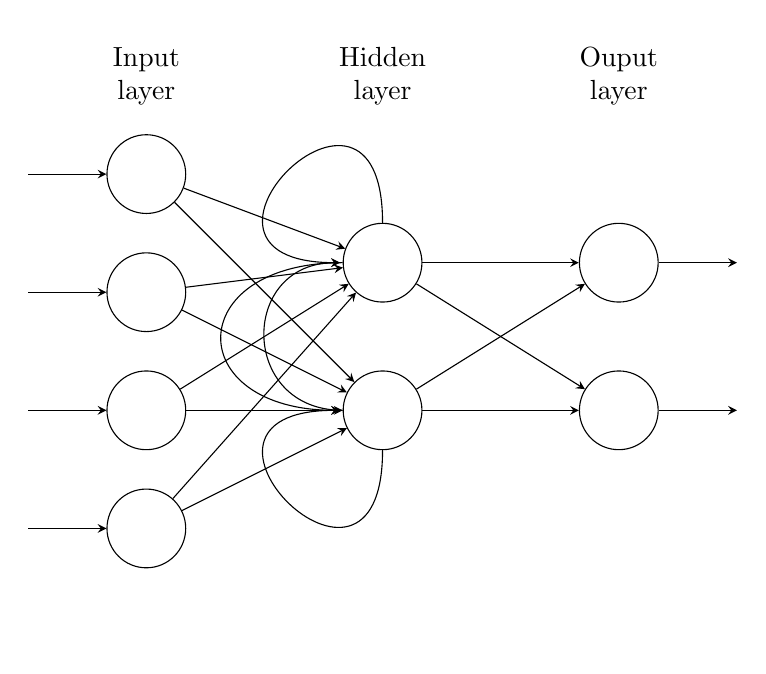
\begin{tikzpicture}[x=1.5cm, y=1.5cm, >=stealth]

\foreach \m/\l [count=\y] in {1,2,3,4}
  \node [every neuron/.try, neuron \m/.try] (input-\m) at (0,2.5-\y) {};

\foreach \m [count=\y] in {1,2}
  \node [every neuron/.try, neuron \m/.try ] (hidden-\m) at (2,2-\y*1.25) {};

\foreach \m [count=\y] in {1,2}
  \node [every neuron/.try, neuron \m/.try ] (output-\m) at (4,2-\y*1.25) {};

\foreach \l [count=\i] in {1,2,3,n}
  \draw [<-] (input-\i) -- ++(-1,0)
    node [above, midway] {};

\foreach \l [count=\i] in {1,n}
  \node [above] at (hidden-\i.north) {};

\foreach \l [count=\i] in {1,n}
  \draw [->] (output-\i) -- ++(1,0)
    node [above, midway] {};

\foreach \i in {1,...,4}
  \foreach \j in {1,...,2}
    \draw [->] (input-\i) -- (hidden-\j);

\foreach \i in {1,...,2}
  \foreach \j in {1,...,2}
    \draw [->] (hidden-\i) -- (output-\j);

\draw[->,shorten >=1pt] (hidden-1) to [out=90,in=180,loop,looseness=8.8] (hidden-1);
\draw[->,shorten >=1pt] (hidden-2) to [out=-90,in=180,loop,looseness=8.8] (hidden-2);

\draw[->,shorten >=1pt] (hidden-1) to [out=180,in=180,loop,looseness=2.8] (hidden-2);
\draw[->,shorten >=1pt] (hidden-2) to [out=180,in=180,loop,looseness=1.8] (hidden-1);


\foreach \l [count=\x from 0] in {Input, Hidden, Ouput}
  \node [align=center, above] at (\x*2,2) {\l \\ layer};

\end{tikzpicture}
\caption{Recurrent Neural Network}
\label{fig:RNN}
\end{center}
\end{figure}
	
	The first paper to advocate for the use of RNNs within the field of network intrusion detection was \cite{debar1992application} in which it was found RNNs to be a promising method of detecting intrusions. A later paper \cite{ryan1998intrusion} re-enforces this statement finding this method to be very effective when employed on real worlds data. Two papers using RNNs in order to detect network intrusions, \cite{tong2009research} and \cite{ghosh1999study} found this approach to have high rate of correct detection of 90\%-100\%, however with a slightly higher false positive rate than other methods of intrusion detection such as the SOM. 
	
	There are however some issues in using RNNs for network intrusion detection. In order to train the network for use in detection, sequenced data such as timed network traffic is required. In this thesis, the data set used is the KDD 1999 Cup dataset in which none of the data is sequenced therefore making it unsuitable for testing with a RNN, which is the main reason why this type of neural network will not be implemented.
	
	\subsubsection{Negative Selection}
	Negative selection is an algorithm in the field of artificial immune systems. Artificial immune systems are a class of algorithm which seek to imitate the immune system of a living creature. \cite{de2002artificial} describes artificial immune systems as \textit{"adaptive systems, inspired by theoretical immunology and observed immune functions, principles and models, which are applied to problem solving."}. There are several algorithms related artificial immune systems such as: Clonal Selection, Immune Network, and Dendritic Cell, however the algorithm which will be examined is the negative selection algorithm. 
	
	The negative selection algorithm takes its inspiration from the generation of T cells in the immune system. These T cells are capable of distinguishing between the bodies own cells and foreign cells, and are created pseudo-randomly. These cells then undergo a censoring process called negative selection in which cells that recognise the body's own cells are destroyed leaving only ones which detect foreign cells. This process is the basis for the negative selection algorithm where detectors (T cells) are generated by some method, randomly or otherwise, and detectors which detect self are deleted \cite{forrest1994self}.
	
	In the negative selection algorithm detectors must be represented by some means. In papers such as \cite{dasgupta1996novelty} and \cite{kim2001towards} detectors are represented by fixed length bit string where each portion of the string is a binary representation of some feature of the input data. In order to determine whether or not these detectors match self, the detector is checked against each entry in the training set and if both of the strings contain the same stretch of \textit{r} uninterrupted bits then the strings are said to match \cite{powers2008hybrid}. The detectors which do not match self are then used to detect intrusive behaviour by attempting to match incoming data represented as bit strings. If the incoming bit string matches any of the detectors it is flagged as intrusive. The use of binary strings as detectors however presents similar problems as found in neural networks. When a string is flagged as being intrusive it is difficult to extract semantic meaning from the detectors, i.e. it is apparent that the string is intrusive but information about what features of the connection made it intrusive are not readily available \cite{gonzalez2003anomaly}. \cite{kim2001evaluation} also found that the use of bit strings for detectors becomes infeasible when using a dataset which contains a lot of different features for each entry, such as in the KDD 1999 Cup dataset.
	A solution to this problem lies in the use of real-valued detectors in the place of bit string detectors. Through the use of real values when defining detectors this allows a great amount of domain knowledge to be extracted from subsequent results. For example when a detector is activated and a connection flagged as being intrusive the detector can be examined and the exact features and values of the connection which triggered the detector can be viewed and higher level information can be extracted. In comparison it can be extremely difficult and time consumting to try and extract semantic knowledge from a bit string as it can be unclear what triggered the detector.
	In order to evolve detectors, there are two main methods of doing so: through random generation, or by means of a genetic algorithm. In the random generation method, a set of self is required, in the form of a dataset of non intrusive behaviour only. Detectors are then generated at random and tested to see whether or not they match the set of self using some method, i.e. r-contiguous bits, r-chunk matching, hamming distance etc. If the generated detector matches self it is discared and a new detector is generated until the detector does not match self and it is stored. Generating detectors by means of a genetic algorithm is described by \cite{powers2008hybrid}. In this paper a population of detectors is initialised where each feature of the detector has a 50\% chance to be initialised as blank and ignored in detection. Leaving fields blank in this way increases the generality of the detector, allowing it to cover as large an area of non-self as possible and to detect more kinds of attacks. The fields which were not left blank during the initialisation are then randomly assigned a value from a list of allowed values for that feature. When evolving the population two parents are bred using a uniform crossover to produce a single child which then has a small probability of mutation. This mutation takes a field from the child and replaces its value with another value which is randomly chosen from the list of allowed values. This newly created child will then replace the parent which it is most similar to if it has a greater fitness. At the end of the evolution process detectors which match self are removed by comparing each detector with the self-set. Generating detectors in such a manner is advantageous as it allows detectors to be created quickly when compared to a purely random generation process.
	
	This method of intrusion detection through the use of the negative selection algorithm has been implemented in a number of papers to great effect. \cite{powers2008hybrid} shows that the negative selection algorithm evolved using a genetic algorithm can acheive detection rates of up to 98\%. \cite{dasgupta2002immunity} found similar results similarly using a genetic algorithm with a self detection rate of 96\% and a non-self detection rate of up to 86\%. This demonstrates that negative selection is an effective and viable method of network intrusion detection.
	
	\subsection{Research Contribution} \label{Research Contribution}
	
During this dissertation the there are a number of goals which are aimed to be met and questions answered in order to ultimatley contribute to the research of network intrusion detection is some way. The main question which is to be answered is what is the difference in performance between a single stage classifier and a two stage classifier in the context of network intrusion detection, and to determine what the configuration of machine learning classifiers discussed within this project produces the highest accuracy network intrusion detection and classification of intrusive network connections, where accuracy is defined as a high number of true positives and a low number of false positives.
	
	Within the field of network intrusion detection there have been numerous papers describing methods of detecting intrusion using single stage classifiers such as {citations} wherein network traffic data is fed into the classifier and the single classifier will determine whether or not the connection is intrusive, and if it is intrusive what class of intrusion it is. Hybrid intrusion detection systems function similarly however the main difference is that there are two stages to the classification process. The first stage will be some form of anomaly detector which reads in network data and determines whether or not a connection is intrusive or not without specifying the type of attack that the intrusive connection is. Then the first stage of the classifier will send all data deemed as intrusive to the second stage of the classifier which will then determine the type of attack. Building an intrusion detection system in a manner such as this allows each stage of the system to specialise in detecting different aspects of a connection and therefore producing a higher detection and classification accuracy. While there have been several papers on hybrid classifiers in the domain of network intrusion detection such as \cite{powers2008hybrid}, \cite{panda2012hybrid}, and \cite{zhang2006hybrid}, there is an apparent distinct lack of papers which directly compare the performance of a single stage monolithic classifier to that of a two-stage stage classifier and investigate different arrangements of machine learning algorithms to evaluate their performance. This gap in research papers is what this dissertation aims to fill.
	
	The project will achieve that goal in the following manner: A number of machine learning algorithms will be chosen to be implemented, i.e. k-nearest neighbors, artificial neural networks, and negative selection. These algorithms will be housed by a peice of software which will be written to run them, obtain metrics and display information on the performance of each algorithm, in the form of tables and graphs, etc. Once this information has been extracted from each algorithm, an analysis and evauluation will be performed on the accuracy of each method, and a conclusion drawn.
		
	\subsection{Dataset}
	The dataset which was to perform the evaluation of the network intrusion detection methods is the KDD Cup 1999 dataset. This dataset comes from the Third International Knowledge Discovery and Data Mining Tools Competition and is based on data captured in the DARPA'98 IDS evaluation program \cite{Lippmann2000darpa}, \cite{tavallaee2009detailed}. 
	
	This dataset has been widely criticized by researchers and experts due to several factors such as; having a large number of redundant records \textit{"which  cause  the  learning  algorithm  to  be  biased  towards  the  most  frequent  records,  thus  prevent  it  from  recognizing  rare  attack  records"} \cite{panda2012hybrid} , and in \cite{vasudevan2011ssenet}, for being outdated meaning that it does not account for new developments in network attacks. This is not of concern during this project as the dataset is used purely as a proof of concept and will not be deployed into an actual network intrusion detection role. There are other datasets which have been proposed for use such as the NSL-KDD which is a revised version of the KDD99 dataset which has been shown to have eliminated many of the faults of the KDD99 dataset while also achieving better performance in the training of network intrusion detection systems \cite{dhanabal2015study}. While all of the criticisms against the KDD Cup 1999 dataset are well founded and a legitimate cause for concern it has been chosen as it is the single most used dataset and researched dataset in the entire network intrusion detection field. With this large amount of research having been performed on this dataset the results from such studies can be used as confirmation that the algorithms which are to be implemented are performing correctly, and also can be used to make an accurate comparisons of results. The KDD Cup 99 dataset also has a version released which has all redundant entries removed while maintaining the correct ratio of non-intrusive entries to attacks, allowing for much faster training of algorithms and collection of data, which is a priority as there is a time constraint which must be followed during this project.
	
	\subsection{Literature Conclusion}
	The research field of Network Intrusion Detection is one of upmost important due to the widespread prevelance of network security breaches and attacks. There have been a large number of studies performed in this area, with each resulting in varying levels of success. The algorithms chosen for this investigation have been proven to be effective at detecting network intrusions, and studies have also shown that through the use of hybrid network intrusion detection systems which make use of multiple classification stages and methods an increase in accurate classification rate. However, machine learning techniques have not yet proven accurate enough in their classification and detection rates to be deployed in a commercial setting, without substantial supervision. There is also a distinct lack within the research in making direct comparisons between different configurations of multiple stage classifiers, and also in making direct comparisons to their single stage counterparts. As a result of this, the conclusion has been reached that conducting an investigation into this area may prove beneficial for future studies, and may provide an insight into what configurations of multiple stage classifiers are effective in the context of network intrusion detection.
